\documentclass[sigconf,edbt]{acmart-edbt2018}

\usepackage{booktabs} % For formal tables


%algorthims
\usepackage{algorithmicx}
%\def\NoNumber#1{{\def\alglinenumber##1{}\State #1}\addtocounter{ALG@line}{-1}}

\usepackage{verbatim} % for multiple line comment
\usepackage[final]{pdfpages} %include pdf files
\usepackage{amsmath}
\usepackage{amssymb}
\mathchardef\mhyphen="2D % Define a "math hyphen" 
\usepackage{amsthm}
\usepackage{eufrak}
\crefname{algocf}{Algorithm}{Algorithms}

\usepackage[ruled,vlined,noend]{algorithm2e}
%algorithm package
\linespread{1.1} % Definition of the linespread
\usepackage[tbtags]{mathtools}
\DeclareMathOperator*{\somefunc}{somefunc}
\SetKwInput{KwInput}{Input}
\SetKwInput{KwOutput}{Output}
\usepackage{algpseudocode}

\usepackage{hyperref}
\usepackage{graphicx}
\usepackage[font=footnotesize]{subfig}

\def\dfar{$\mathit{DFA_{R}}$}
\def\nfar{$\mathit{NFA_{R}}$}
\def\dfasr{$\mathit{DFA_{\Sigma^{*}\cdot R}}$}
\def\nfasr{$\mathit{NFA_{\Sigma^{*}\cdot R}}$}
\def\pmcmr{$\mathit{PMC_{R}^{m}}$}
\def\pmczeror{$\mathit{PMC_{R}^{0}}$}
\def\pmconer{$\mathit{PMC_{R}^{1}}$}
\def\pfc{$\mathit{P_{fc}}$}


\usepackage{listings}
\usepackage{color}

\definecolor{dkgreen}{rgb}{0,0.6,0}
\definecolor{gray}{rgb}{0.5,0.5,0.5}
\definecolor{mauve}{rgb}{0.58,0,0.82}

\lstset{
	language=Java,
	aboveskip=3mm,
	belowskip=3mm,
	showstringspaces=false,
	columns=flexible,
	basicstyle={\small\ttfamily},
	numbers=none,
	numberstyle=\tiny\color{gray},
	keywordstyle=\color{blue},
	commentstyle=\color{dkgreen},
	stringstyle=\color{mauve},
	breaklines=true,
	breakatwhitespace=true,
	tabsize=3,
	captionpos=b
}


% Copyright
\setcopyright{rightsretained}

\usepackage[inline,shortlabels]{enumitem}
% DOI
\acmDOI{}

% ISBN
\acmISBN{978-3-89318-078-3}

%Conference
\acmConference[EDBT 2018]{21st International Conference on Extending Database Technology (EDBT)}{March 26-29, 2018}{Vienna, Austria} 
\acmYear{2018}

\settopmatter{printacmref=false, printccs=false, printfolios=false}

\pagestyle{plain} % removes running headers


\begin{document}
\title{A Distributed Online Learning Approach for Pattern Prediction over Movement Event Streams with Apache Flink - DRAFT}

%\title{Leveraging Distributed Online Learning For Pattern Prediction over Movement Event Streams with Apache Flink}
%
%\titlenote{Produces the permission block, and copyright information}
%\subtitle{Extended Abstract}
%\subtitlenote{The full version of the author's guide is available as
 % \texttt{acmart.pdf} document}
  
\author{Ehab Qadah}
\affiliation{%
	\institution{Fraunhofer IAIS}
	\streetaddress{Schloss Birlinghover}
	\city{Sankt Augustin} 
	\country{Germany} 
	\postcode{43017-6221}
}
\email{Ehab.Qadah@iais.fraunhofer.de}

\author{Michael Mock}
\affiliation{%
	\institution{Fraunhofer IAIS}
	\streetaddress{Schloss Birlinghover}
	\city{Sankt Augustin} 
	\country{Germany} 
	\postcode{43017-6221}
}
\email{Michael.Mock@iais.fraunhofer.de}


\author{Elias Alevizos}
\affiliation{%
	\institution{NCSR "Demokritos"}
	\streetaddress{}
	\city{Athens} 
	\country{Greece} 
	\postcode{43017-6221}
}
\email{alevizos.elias@iit.demokritos.gr}

\author{Georg Fuchs}
\affiliation{%
  \institution{Fraunhofer IAIS}
  \streetaddress{Schloss Birlinghover}
  \city{Sankt Augustin} 
  \country{Germany} 
  \postcode{43017-6221}
}
\email{Georg.Fuchs@iais.fraunhofer.de}

\renewcommand{\shortauthors}{}


\begin{abstract}
We present a distributed online prediction system for user-defined patterns over multiple massive streams of events related to trajectories of movement objects, built using the general purpose stream processing framework Apache Flink. The proposed approach is based on combing probabilistic event pattern prediction models on multiple predictor nodes with a distributed online learning protocol in order to continuously learn a global prediction model to share it among the predictors in a communication-efficient way. Our approach enables the  collaborative learning between the predictors (i.e., "learn from each other"), thus the learning rate is accelerated. The underlying model provides an online predictions when a pattern (i.e., a regular expression over the event types) will be completed within each event stream. We describe the distributed architecture of the system, its implementation in Flink, and present some empirical evaluation results over real-world event streams related to trajectories of moving vessels.

\end{abstract}

\keywords{Big Movement Event Streams, Stream Processing, Event Pattern Prediction, Distributed Pattern Markov Chain.}

\maketitle


\section{INTRODUCTION}


\par In recent years, technological advances have led to a growing availability of massive amounts of continuous streaming data (i.e., data streams observing events) in many application domains such as social networks \cite{mathioudakis2010twittermonitor}, Internet of Things (IoT) \cite{miorandi2012internet}, and maritime surveillance \cite{patroumpas2015event}.  The ability to detect and predict the full matches of a pattern of interest (e.g., a certain sequence of events), defined by a domain expert, is typically important for operational decision making tasks in the respective domains.

\par An event stream is an unbounded collection of time-ordered data observations in the form of a tuple of attributes that is composed of a value from finite event types along with other categorical and numerical attributes. In this work, we deal with movement event streams. For instance, in the context of maritime surveillance, the event stream of a moving vessel consists of spatiotemporal and kinematic information along with the vessel's identification and its trajectory related events, based on the automatic identification system (AIS) \cite{ais} messages that are continuously sent by the vessel. Therefore, leveraging event patterns prediction over real-time streams of moving vessels is useful to alert maritime operation managers about suspicious activities (e.g., fast sailing vessels near ports, or illegal fishing) before they happen. However, processing real-time streaming data with low latency is challenging, since data streams are large and distributed in nature and continuously arrive at a high rate. 
% we describe the design and implementation of a system called% 
\par In this paper, we present the design and implementation of an online, distributed and scalable pattern prediction system over multiple, massive streams of events. More precisely, we consider event streams related to trajectories of moving objects (i.e., vessels). The proposed approach is based on a novel method that combines a distributed online prediction protocol \cite{dekel2012optimal,kamp2014communication} with an event forecasting method based on Markov chains \cite{alevizos2017event}. It is implemented on top of the Big Data framework for stream processing Apache Flink \cite{Flink}. We evaluate our proposed system over real-world data streams of moving vessels, which are provided in the context of the datAcron project\footnote{\url{http://www.datacron-project.eu/}}.

\par The rest of the paper is organized as follows. We discuss the related work and used frameworks in Section ~\ref{sec:realred_work}. In Section ~\ref{sec:system}, we describe the problem of pattern prediction, our proposed approach, and the architecture of our system. The implementation details on top of Flink are presented in Section ~\ref{sec:impl} and the experimental results in Section ~\ref{sec:results}. We conclude in Section ~\ref{sec:concl}.


\section{RELATED WORK AND BACKGROUND}
\label{sec:realred_work}
\subsection{Related work}


\subsection{Pattern prediction over event streams}


\subsubsection*{Related work:\\}
The task of forecasting over time-evolving streams of data can be formulated in various different ways and with varying assumptions.
One of the most usual ways to formalize this task is to assume that the stream is a time-series of numerical values and the goal is to forecast at each time point $n$ the values at some future points $n+1$, $n+2$, etc. (or even the output of some function of future values). 
This is the task of time-series forecasting \cite{montgomery_introduction_2015}.
Another way to formalize this task is to view streams as sequences of events,
i.e., tuples with multiple, possibly categorical, attributes, like \textit{event type}, \textit{timestamp}, etc. 
In this work that we present here, 
we focus on this latter definition of forecasting (event forecasting).  A substantial body of work on event forecasting comes from the field of temporal pattern mining where events are defined as 2-tuples of the form $(\mathit{EventType},\mathit{Timestamp})$.
The ultimate goal is to extract patterns of events in the form either of association rules \cite{agrawal_mining_1993} or frequent episode rules \cite{mannila_discovery_1997}. 
These methods have been extended in order to be able to learn not only rules for detecting event patterns but also rules for predicting events.
For example, in \cite{vilalta_predicting_2002}, a variant of association rule mining is where the goal is to extract sets of event types that frequently lead to a rare, target event within a temporal window. 
In \cite{laxman_stream_2008}, a probabilistic model is presented
in order to calculate the probability of the immediately next event in the stream. 
This is achieved by using standard frequent episode discovery algorithms and combining them with Hidden Markov Models and mixture models.
The framework of episode rules is employed in \cite{fahed_efficient_2014} as well.
The output of the proposed algorithms is a set predictive rules whose antecedent is minimal (in number of events) and temporally distant from the consequent.
In \cite{zhou_pattern_2015} a set of algorithms is proposed that target batch, online mining of sequential patterns, without maintaining exact frequency counts.
As the stream is consumed, the learnt patterns can be used to test whether a prefix matches the last events seen in the stream, 
indicating a possibility of occurrence for events that belong to the suffix of the rule.

Event forecasting has also attracted some attention from the filed of Complex Event Processing (see \cite{Cugola:2012:PFI:2187671.2187677} for a review).
One such early approach is presented in \cite{muthusamy_predictive_2010}.
Complex event patterns are converted to automata and subsequently
Markov chains are used in order to estimate when a pattern is expected to be fully matched.
A similar approach is presented in \cite{alevizos2017event},
where again automata and Markov chains are employed in order to provide (future) time intervals during which a match is expected with a probability above a confidence threshold. 

\subsubsection*{Event forecasting with pattern Markov Chains:\\}

For our work presented in this paper,
we use the approach described in \cite{alevizos2017event}.
For the sake of self-containment,
we briefly describe this approach in what follows.

The problem at hand may be stated as follows: given a stream of low-level events and a pattern defining relations between low-level events, 
in the form of a regular expression (i.e., using operators for \textit{sequence}, \textit{disjunction} and \textit{iteration}),
the goal is to estimate at each new event arrival the number of future events
that we will need to wait for until the expression is satisfied (and therefore a match be detected).

As a first step, event patterns are converted to deterministic finite automata (DFA) through standard conversion algorithms.
As an example, see Figure \ref{fig:dfatcc} for the DFA of the simple sequential pattern $R=a\cdot c\cdot c$ and an alphabet $\Sigma=\{a,b,c\}$
(note that the DFA has no dead states since we need to handle streams and not strings).
The next step is to derive a Markov chain that will be able to provide a probabilistic description of the DFA's run-time behavior.
Towards this goal, we use Pattern Markov Chains, as  proposed in \cite{nuel_pattern_2008}.
Under the assumption that the input events are independent and identically distributed (i.i.d.), it can be shown that there is a direct mapping of the states of the DFA to states of a Markov chain and the transitions of the DFA to transitions of the Markov chain.
The transition probabilities of the Markov chain are the occurrence probabilities of the various event types.
On the other hand, if the occurrence probabilities of the events are dependent on some of the previous events seen in the stream 
(i.e., the stream is generated by an $m^{th}$ order Markov process),
we might need to perform a more complex transformation 
(see \cite{nuel_pattern_2008} for details)
in order to obtain a ``proper'' Markov chain.
The transition probabilities are then conditional probabilities on the event types.
In any case,
we call such a derived Markov chain a Pattern Markov Chain (PMC) of order m
and denote by \pmcmr , where $R$ is the initial pattern and $m$ the assumed order.
As an example, see Figure \ref{fig:mctcc1}, which depicts the PMC of order 1 for the DFA of Figure \ref{fig:dfatcc}.
%\begin{comment}
\begin{figure}[!ht]
\begin{centering}
\subfloat[\dfasr]{
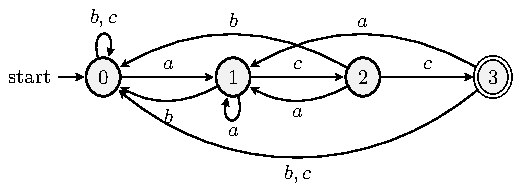
\includegraphics[height=0.105\textheight,width=\linewidth]{./figures/forecasting/dfasr.pdf}
\label{fig:dfatcc}
}
\hfill
\subfloat[\pmconer]{
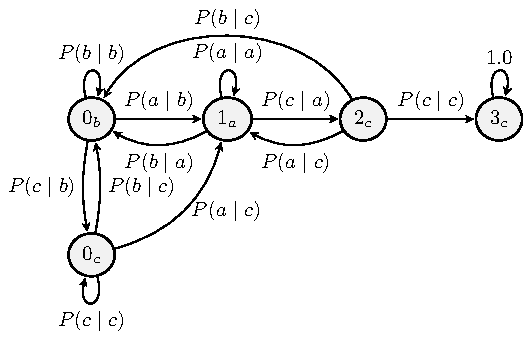
\includegraphics[width=0.35\textwidth]{./figures/forecasting/pmcr1.pdf}
\label{fig:mctcc1}
}
%\hfill
\caption{DFA and PMC for $R=a\cdot c\cdot c$,  $\Sigma=\{a,b,c\}$ and $m=1$.}
\label{fig:dfa_mc_example}
\end{centering}
\end{figure}
%\end{comment}


After constructing a PMC, we can use it in order to calculate the so-called \textit{waiting-time} distributions.
Given a specific state of the PMC, a \textit{waiting-time} distribution gives us the probability of reaching a set of absorbing states in $k$ transition from now (absorbing states are states with self-loops and probability equal to $1.0$).
By mapping the final states of the initial DFA to absorbing states of the PMC
(see again Figure \ref{fig:dfa_mc_example}),
we can therefore calculate the probability of reaching a final state,
or, in other words, of detecting a full match of the original regular expression in $k$ events from now.

In order to estimate the final forecasts, another step is required,
since our aim is not to provide a single future point with the highest probability but an interval. 
Forecasts are given in the form of intervals, like $I=(\mathit{start},\mathit{end})$. 
The meaning of such an interval is that the DFA is expected to reach a final state sometime in the future between $\mathit{start}$ and $\mathit{end}$ with probability at least some constant threshold $\theta_{fc}$ (provided by the user). 
These intervals are estimated by a single-pass algorithm that scans a waiting-time distribution and finds the smallest (in terms of length) interval that exceeds this threshold. 
An example is shown in Figure \ref{fig:wtdfas},
where the DFA in Figure \ref{fig:dfa1} is in state $1$,
the \textit{waiting-time} distributions for all of its non-final states are shown in Figure \ref{fig:wt1}
and the distribution, along with the forecast interval, for state $1$ are shown in green.
\begin{figure}[!ht]
\begin{centering}
\subfloat[DFA, state 1.]{ 
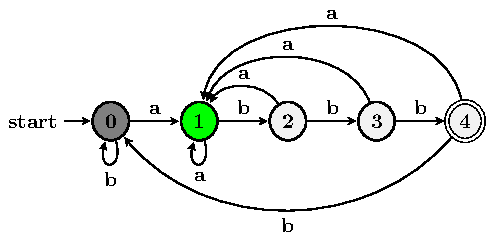
\includegraphics[width=0.15\textwidth,height=0.12\textheight]{./figures/forecasting/dfa1.pdf}
\label{fig:dfa1}
}
\subfloat[Waiting-time distribution, state 1.]{ 
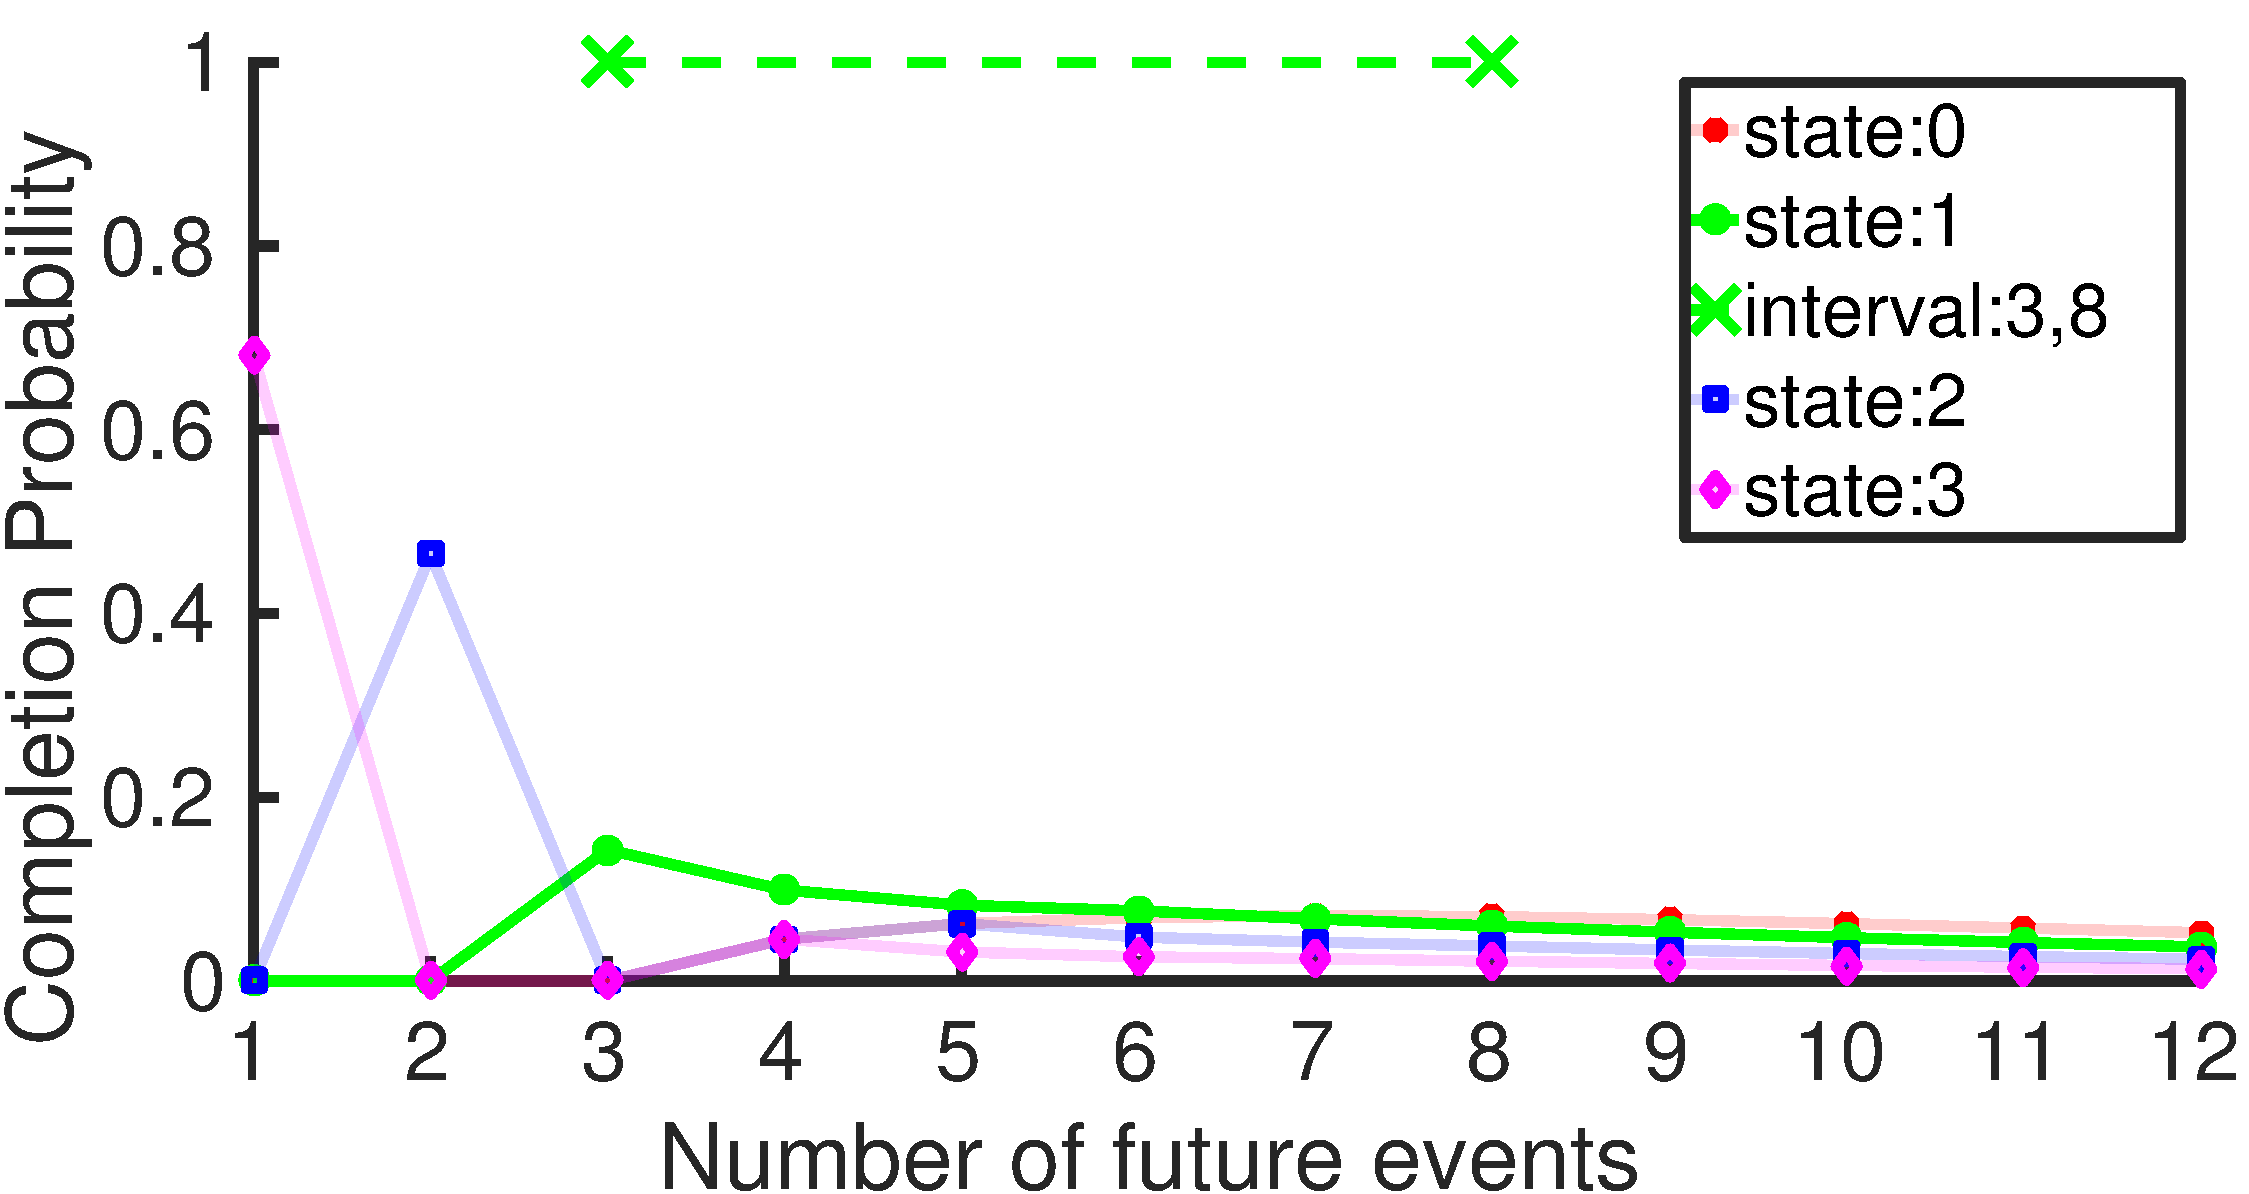
\includegraphics[width=0.3\textwidth,height=0.16\textheight]{./figures/forecasting/wt1.pdf}
\label{fig:wt1}
}
\caption{Example of how forecasts are produced. 
$R=a\cdot b\cdot b\cdot b$, $\Sigma=\{a,b\}$, $m=1$, $\theta_{\mathit{fc}}=0.5$.}
\label{fig:wtdfas}
\end{centering}
\end{figure}

The above described method assumes that we know the (possibly conditional) occurrence probabilities of the various event types appearing in a stream
(as would be the case with synthetically generated streams).
However, this is not always the case in real-world situations.
Therefore, it is crucial for a system implementing this method to have the capability to learn the values of the PMC's transition matrix.
One way to do this is to use some part of the stream to obtain the maximum-likelihood estimators for the transition probabilities. 
If $\boldsymbol{\Pi}$ is the transition matrix of a Markov chain with a set of states $Q$, 
$\pi_{i,j}$ the transition probability from state $i$ to state $j$,
$n_{i,j}$ the number of transitions from state $i$ to state $j$,
then the maximum likelihood estimator for $\pi_{i,j}$ is given by:
\begin{equation*}
\label{eq:pi_estim}
\hat{\pi}_{i,j}=\frac{n_{i,j}}{\sum_{k \in Q} n_{i,k}}=\frac{n_{i,j}}{n_{i}}
\end{equation*}
Executing this learning step on a single node might require a substantial amount of time until we arrive at a sufficiently good model.
In this paper, we present a distributed method for learning the transition matrix.


\subsubsection*{Distributed Online Learning}
\par In recent years, the problem of distributed online learning has received increased attention and has been studied in \cite{langford2009slow,yan2013distributed,xiao2010dual,dekel2012optimal,kamp2014communication}.  A distributed online mini-batch prediction approach over multiple data streams has been proposed in \cite{dekel2012optimal}. This approach is based on a static synchronization method. The learners periodically communicate  their local models with a central coordinator unit after consuming a fixed number of input samples/events (i.e., batch size $b$), in order to  create a global model and share it between all learners. This work has been extended in \cite{kamp2014communication} by introducing a
dynamic synchronization scheme that reduces the required communication overhead. It can do so by making the local learners communicate their models only if they diverge from a reference model. In this work, we employ this protocol with event patterns prediction models over multiple event streams. 

\subsection{Technological Background}

\par In the last years, many systems for large-scale and distributed stream processing have been proposed, including Spark Streaming \cite{Spark},  Apache Storm \cite{Storm} and Apache Flink \cite{Flink}. These frameworks can ingest and process real-time data streams, published from different distributed message queuing platforms, such as Apache Kafka \cite{Kafka} or  Amazon Kinesis \cite{Kinesis}. In this work, we implemented the proposed system in Apache Flink and Apache Kafka (see Section ~\ref{sec:impl}).

% Flink provides the distributed stream processing components of the distributed event pattern predictors. It works alongside Apache Kafka,
%which is used for streaming the input event streams and as a messaging platform to enable the distributed online learning functionalities.


\par In the datAcron project, the Flink streaming processing engine has been chosen as a primary platform for supporting the streaming operations, based on an internal comparative evaluation of several streaming platforms. Hence, we used it to implement our system. A predecessor distributed online learning framework has already been implemented in the FERARI project \cite{flouris2016ferari} based on Apache Storm.


% In Storm, a distributed application is expressed as a "topology", in which the individual processing steps called "Bolts" are connected
%in a data workflow. This means, that each Bolt can is sending and receiving data streams from other Bolts, for example, there are bolts generating
%the local models for each incoming data streams and there is a Bolt representing the "Coordinator" for executing the synchronization protocol between
%the local models. As the synchronization protocol includes the steps of sending the local models to the coordinator (for merging the models) and of sending
%the merged model back, it results in a cyclic workflow structure, which is supported in Storm. 

\subsubsection*{Apache Flink}

\par Apache Flink is an open source project that provides a large-scale, distributed, and stateful stream processing platform \cite{carbone2015apache}. Flink is one of the most recent and pioneering Big Data processing frameworks. It provides processing models for both streaming and batch data, where the batch processing model is treated as a special case of the streaming one (i.e., finite stream). Flink's software stack includes the \textit{DataStream} and \textit{DataSet} APIs for processing infinite and finite data, respectively. These two core APIs are built on top of Flink's core dataflow engine and provide operations on data streams or sets such as mapping, filtering, grouping, etc.

\par The two main data abstractions of Flink are \textit{DataStream} and \textit{DataSet},  they represent read-only collections of data elements. The list of elements is bounded (i.e., finite) in \textit{DataSet}, while it is unbounded (i.e., infinite) in the case of \textit{DataStream}. Flink's core is a distributed streaming dataflow engine. Each
Flink program is represented by a data-flow graph (i.e., directed acyclic graph - DAG) that gets executed by Flink's dataflow engine \cite{carbone2015apache}. The data flow graphs are composed of stateful operators and intermediate data stream partitions.  The execution of each operator is handled by multiple parallel instances whose number is determined by the \textit{parallelism} level. Each parallel operator instance is executed in an independent task slot on a machine within a cluster of computers \cite{Flink}.    

\subsubsection*{Apache Kafka}

\par Apache Kafka is a scalable, fault-tolerant, and distributed streaming framework/messaging system \cite{Kafka}. It allows to publish and subscribe to arbitrary data streams, which are managed in different categories (i.e., \textit{topics}) and  partitioned in the Kafka cluster. The Kafka Producer API provides the ability to publish a stream of messages to a topic. These messages can then be consumed by applications, using the Consumer API that allows them to read the published data stream in the Kafka cluster. In addition, the streams of messages are distributed and load balanced between the multiple receivers within the same consumer group for the sake of scalability.
  





%The distributed online learning framework has already been implemented in the FERARI  distributed streaming architecture based on Storm. 
%In Storm, a distributed application is expressed as a so-called “topology”, in which the individual processing steps called “Bolts” are connected
%in a data workflow. This means, that each Bolt can is sending and receiving data streams from other Bolts, for example, there are bolts generating
%the local models for each incoming data streams and there is a Bolt representing the “Coordinatior” for executing the synchronisation protocol between
%the local models. As the synchronisation protocol includes the steps of sending the local models to the coordinator (for merging the models) and of sending
%the merged model back, it results in a cyclic workflow structure, which is supported in Storm. 
%
%Why Flink
%In the Datacron project, the Flink streaming engine has been chosen as primary platform for supporting the streaming operations, based on an internal comparative evaluation of several streaming platforms
%regarding functionality and performance. We will discuss in section.. how to implement the required communication structure for the distributed
%online learning framework in Flink.

\section{SYSTEM OVERVIEW}
\subsection{Problem Formulation}
%refine the stream and event pattern %
%define the pattern we deal formally%
% include base line 1 batch size in experemintal results%

We follow the terminology of \cite{luckham2008power,alevizos2015complex,zhou2015pattern} to formalize the problem we tackle. Given a set of \emph{$K$} real-time streams of events $S = \{ s_1,s_2, ..., s_k\}$ as input, which are associated with a set of $K$  objects $O = \{ o_1, ..., o_k\}$. Where each stream $s_i=\langle e_1,e_3,...,e_t,...\rangle$  is a time-ordered sequence of events, these events are connected to a moving object  $o_i \in O$,  $e_t$  refers to the current time event within the unbounded stream, we give the definition of the input event sample as follows:  
\begin{definition}
	Each event is defined as a tuple of attributes $$e_i = (type,\tau,a_1,a_2.....,a_n,id)$$ Where $type$ is the event type attribute that takes a value from a set of finite event types/symbols $\Sigma$, $\tau$ represents the timestamp of the event tuple,  the  $a_1,a_2,...,a_n$ are spatial or other contextual features (e.g., speed); these features are varying from one application domain to another, while the $id$ attribute connects the event tuple to an associated moving object.
\end{definition}

A user-defined pattern $\mathcal{P}$ is given in the form of regular expression over $\Sigma$ (i.e., event types) \cite{alevizos2017event}, and the main goal is to predict the full matches of $\mathcal{P}$ within each event stream $s_i\in S$ in real-time.

\par The setting that is considered in this work is described in the following:\\
A large-scale patterns prediction over multiple input event streams system that  consists of $K=\left\vert{S}\right\vert$ distributed predictor nodes $n_1,n_2...,n_k$, each of which consumes an input event stream $s_i\in S$, and provides an online predication service. Each node $i \in [K]$ handles a single event stream $s_i$ associated with a moving object $o_i \in O$, in addition,  it  maintains a local prediction model $f_i$ for the user-defined pattern $\mathcal{P}$. An online prediction about the future full match of the pattern $\mathcal{P}$ in $s_i$ is provided for each new arriving event tuple. In summary, we have multiple running instances of an online prediction algorithm on distributed nodes for multiple input event streams, each instance provides online predications about a pre-defined pattern of events.  We consider as input a massive event streams that describe trajectories of  moving objects, more specifically, event streams of moving vessels in the context of maritime surveillance.  

The defined pattern $\mathcal{P}$ is monitored over each event stream $s_i$  by a  predictor nodes  $n_i$  that maintains a local prediction model $f_i$, where there is one node for each vessel's event stream.  The prediction model $f_i$ gives the ability to provide an online predictions about when the pattern will be completed in the form of an expected number of future events before a full match does occur.

\subsection{The Proposed Approach}
\label{sec:proposed_approach}
\par We design and develop a scalable and distributed patterns prediction system over massive input event streams of moving objects. We  exploit the event forecasting with Pattern Markov Chains \cite{alevizos2017event} as the base prediction model (i.e., $f_i$). Moreover,  we propose to enable the information exchange between the distributed predictors/learners of the input event streams, by adapting the distributed online predication protocol \cite{dekel2012optimal,kamp2014communication} to synchronize the prediction models, i.e., Markov transitions probabilities of the Pattern Markov Chain (PMC) predictors.

\par We propose a $synchronization operation$  for the distributed Pattern Markov Chain (PMC) models based on the maximum-likelihood estimation \citep{anderson1957statistical} for the transition probabilities matrix of the underlying Markov Chain described by: 
\begin{equation}
\label{eq:pi_estim}
\hat{p}_{i,j}=\frac{\sum_{k \in K} n_{k,i,j}}{\sum_{k \in K} \sum_{l \in L} n_{k,i,l}}
\end{equation}


\par Our approach relies on enabling the collaborative learning between the prediction models of  the input event streams. By doing so, we assume that the underlying event streams belong to the same  distribution and share the same behavior (e.g., mobility patterns). We claim that assumption is reasonable in many application domains, for instance, in the context of maritime surveillance, vessels travel through defined routes by International Maritime Organization (IMO). Additionally, vessels have similar mobility patterns in specific areas such as moving with low speed and multiple turns near the ports \cite{pallotta2013vessel,liu2014knowledge}. That allows our system to dynamically construct a coherent global prediction model for all input event streams based on merging its local models.

\par By enabling collaborative learning our approach is imposing an acceleration of learning of the underlying prediction models with less training data, in addition, it provides an improvement of the predictive performance compared to the no-distributed  version of event forecasting with Pattern Markov Chains system. 


\subsection{Distributed Architecture}
\label{sec:architecture}
Our system consumes an aggregated events stream as input\footnote{In practice, the aggregated input events stream is composed of multiple input event streams for multiple moving objects, which are reconstructed bt the system internally.} of large number of moving objects, which is continuously collected and fed into the system. It allows users to register a pattern $\mathcal{P}$ to be monitored over each event stream of a moving object. Output stream consists of original input events alongside with predictions of full matches of $\mathcal{P}$ is outputted to be displayed to the end users. Figure ~\ref{fig:architecture} presents the overview of our system architecture and its main components.      


\begin{figure}[h]

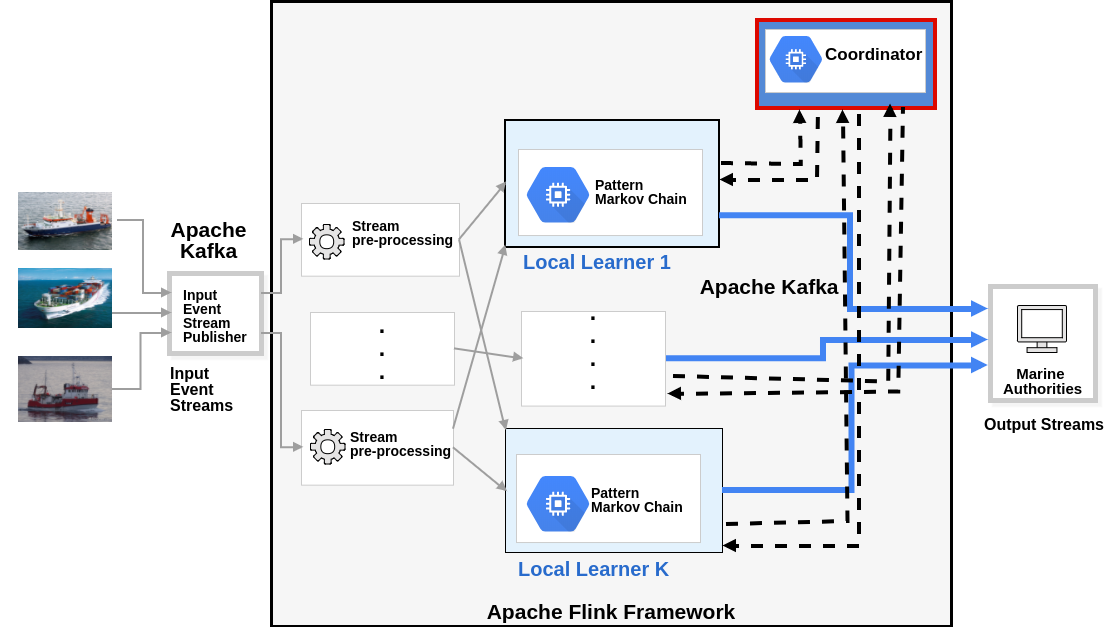
\includegraphics[height=2.5in, width=\linewidth]{figures/distributed_architecture.png}
	
\caption{System Architecture.}
\label{fig:architecture}
\end{figure}

The system is composed of three processing units:   \begin{enumerate*}[(i)]
	\item pre-processing operators that receive the input event stream, and perform filtration, ordering operations, before partitioned the input event stream to multiple event streams based on the associated moving object 
	\item predictor nodes (learners), which are responsible to maintain a prediction model for the input event streams, such that each prediction node is configured to handle an event stream from the same moving object, in order to provide online predictions for a predefined pattern $\mathcal{P}$  
	\item a coordinator node that communicates through a Kafka stream channels with the predictors to realize the distributed online learning protocol, which builds a global prediction model based on the received local models, and then share it among the predictors.
\end{enumerate*}

\par In summary, our distributed system consists of multiple pre-processing operators, prediction nodes,  and a central coordinator node. All units are running concurrently and arranged as data processing pipeline as depicted in Figure ~\ref{fig:architecture}. We leverage the Apache Kafka as messaging system to ingest the input event streams and to publish the result streams, in addition, it used as the communication channel between the predictor nodes and the coordinator. While Apache Flink is employed to execute the system's distributed processing units over the input event streams. Our system architecture can be modeled as logical network of processing nodes  organized in a Directed Acyclic Graph (DAG), which is inspired by the Flink runtime dataflow programs \cite{carbone2015apache}.  



\section{IMPLEMENTATION DETAILS}
\label{sec:impl}
This sections provides a detailed overview of the system's implementation, our system has been implemented on top of Apache Flink and Apache Kafka frameworks. Each of the three sub-modules described in Section  ~\ref{sec:architecture} have been implemented as Flink operations over the input events stream. 

\textbf{Pre-processing and Prediction Operators.} Listing ~\ref{algonline:flink1} shows how the workflow of the system is implemented as data flow in Flink program.


	\begin{lstlisting}[caption={Flink pipeline for local predictors workflow},label={algonline:flink1},frame=single]
	.....
	DataStream<Event> inputEventsStream = env.addSource(flinkKafkaConsumer);	
	// Create event tuples (id,event) and assign time stamp 
	DataStream<Tuple2<String, sEvent>> eventTuplesStream =
	inputEventsStream.map(new EventTuplesMapper())
	.assignTimestampsAndWatermarks(new EventTimeAssigner());	
	// Create the ordered keyed stream 
	KeyedStream<Tuple2<String, Event>, Tuple> keyedEventsStream =
	eventsStream.keyBy(0).process(new EventSorter())
	.keyBy(0);	
	//Initialize the predictor node 
	LocalPredictorNode predictorNode =new LocalPredictorNode<Event>(P);
	// Process the  keyedEventsStream by the predictor 
	DataStream<Event> processedEventsStream =
	keyedEventsStream.map(predictorNode);
	...
	\end{lstlisting}
	
The system ingests the input events stream form a Kafka cluster that mapped to \textbf{DataStream} of events, which is then processed by a \textbf{EventTuplesMapper} to create tuples of (id,event), where the  \textbf{id} is associated moving object id. And in order to manage the out of order incoming events the tuples stream is processed by a \textbf{TimestampAssigner} that assigns the timestamps for the input events  based on the extracted creation time. Afterward,  an ordered stream of event tuples is generated using a process function \textbf{EventSorter}. The ordered stream is transformed to a \textbf{keyedEventsStream} based on partitioning it based on the ids of the associated moving object using a \textbf{keyBy} operator. A local \textbf{predictor} node in a distributed environment is represented by a \textbf{map} function over the \textbf{keyedEventsStream} that internally maintains a single prediction model (i.e., pattern markov chain predictor) per each \textbf{id} using the Flink's Keyed State \footnote{\url{https://ci.apache.org/projects/flink/flink-docs-release-1.3/dev/stream/state.html\#keyed-state}}. The output streams of the moving objects form the predictor map parallel instances are sent to a new Kafka stream (i.e., same topic name) that can be processed by other components like visualization or users notifier.


\par Moreover, the implementation of  a \textbf{predictor} map function includes the communication  with \textbf{coordinator} using Kafka streams. At the beginning of the execution it sends a reregistration request to the coordinator. And at runtime it sends  its local prediction model as synchronization request,  or as a response for a resolution request from the coordinator. In addition, it receives a resolution request from the coordinator to send its model. These communication messages are published onto different  Kafka topics as depicted in Table~\ref{tab:messagesToTopics}. 

\begin{table}[h]
	\caption{Message to Kafka topics mapping.}
	\label{tab:messagesToTopics}
	\begin{tabular}{p{3cm}l}
		\toprule
		Message &Kafka Topic\\
		\midrule
		\parbox[t]{4cm}{\textbf{RegisterNode}, \\ \textbf{RequestSync} and \\\textbf{ResolutionAnswer} } &LocalToCoordinatorTopicId\\ \\
		
			  \parbox[t]{4cm}{\textbf{CoordinatorSync} and \\ \textbf{RequestResolution}} &CoordinatorToLocalTopicId\\
		
		\bottomrule
	\end{tabular}
\end{table}


\textbf{Coordinator.} Listing ~\ref{algonline:flink2} presents the workflow of the coordinator node that manages the distributed online learning protocol operations, which is implemented as Flink program. The coordinator receives messages from the local predictors through a Kafka Stream of a topic named \textbf{"LocalToCoordinatorTopicId"}, while it is implemented as a single \textbf{map} function over the messages stream by setting the \textbf{parallelism} level of the Flink program to \textbf{"1"} \footnote{Increasing the parallelism will scale up the number of parallel coordinator instances, but for the current setting a single node in needed.}. The coordinator map operator handles three type of messages from the predictors: \begin{enumerate*}[(i)]
	\item \textbf{RegisterNode} that contains  a registration request for a new predictor instance,
	\item \textbf{RequestSync} to receive a local model of a predictor node after violation,
	\item \textbf{ResolutionAnswer} to receive a resolution response from  a local predictor node.  
\end{enumerate*}  
 While it sends \textbf{CoordinatorSync} messages for all predictors after creating a new global prediction model, or \textbf{RequestResolution} to a ask the local predictors for their prediction models.
 

\begin{lstlisting}[caption={The coordinator Flink program.},label={algonline:flink2},frame=single]
...
	StreamExecutionEnvironment env = .......;
	env.setParallelism(1);
 
	// Read messages from local predictors
	DataStream<TopicMessage> messagesStream = readKafkaStream(env, "LocalToCoordinatorTopicId");
	
	// Initialize the coordinator node
	CompunctionEfficientCoordinator coordinatorNode = new CompunctionEfficientCoordinator(configs);
	
	DataStream<CoordinatorMessage> coordinatorMessagesStream = messageStream.map(coordinatorNode);
	
	// Send the messages form the coordinator to the local predictors
	writeKafkaStream(coordinatorMessagesStream, CoordinatorToLocalTopicId);

...
\end{lstlisting}

                 


\section{EMPIRICAL EVALUATION}
\label{sec:results}
In this section, we present experimental results on real-world event streams in the context of maritime and aviation domains provided by the datAcron project.

\section{CONCLUSION}
\label{sec:conclusion}

\begin{acks}
	
	This work was supported by the EU H2020 datAcron project (grant agreement No 6875).
	
\end{acks}

\bibliographystyle{ACM-Reference-Format}
\bibliography{bmda-paper-bibliography,forecasting} 


\end{document}
